%        File: chameleon-arch.tex
%     Created: Mon Jan 04 02:00 PM 2016 C
% Last Change: Mon Jan 04 02:00 PM 2016 C
%
\documentclass{standalone}

\usepackage{tikz}
\usetikzlibrary{positioning, shapes, calc, backgrounds, fit}

\begin{document}
\begin{tikzpicture}[magnify/.style = {dashed, blue, ultra thick}, 
  connection/.style = {<->, blue, line width = 3pt}]
  % background: china map
  \node (china-map) [opacity = 0.20] {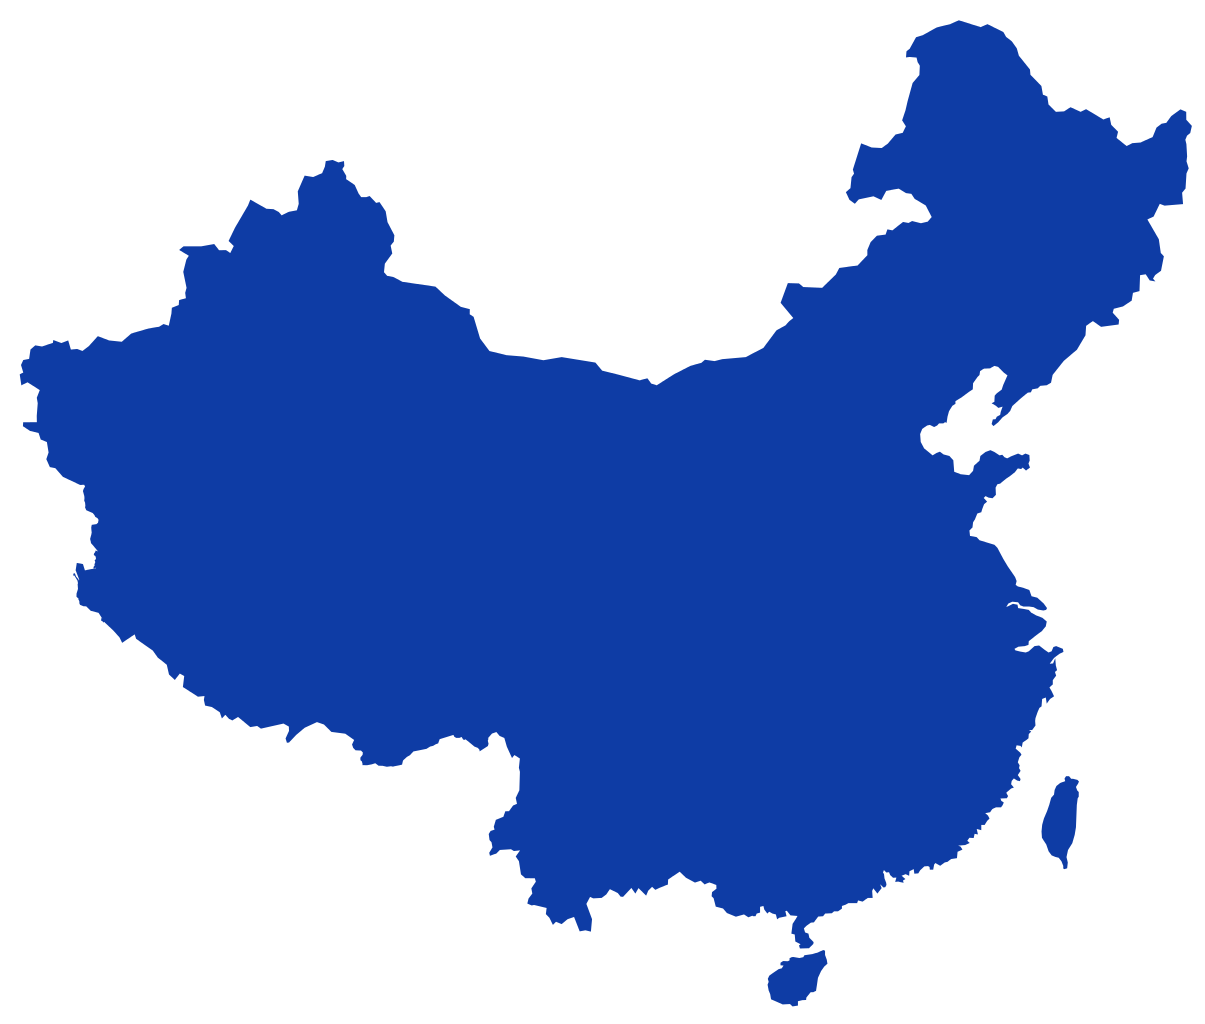
\includegraphics[scale = 0.40]{figs/china-outline-blue.png}};
  % master-slave-left, master-slave-right, and master-slave-below
  \node (master-slave-left) [] at (-6, 1) {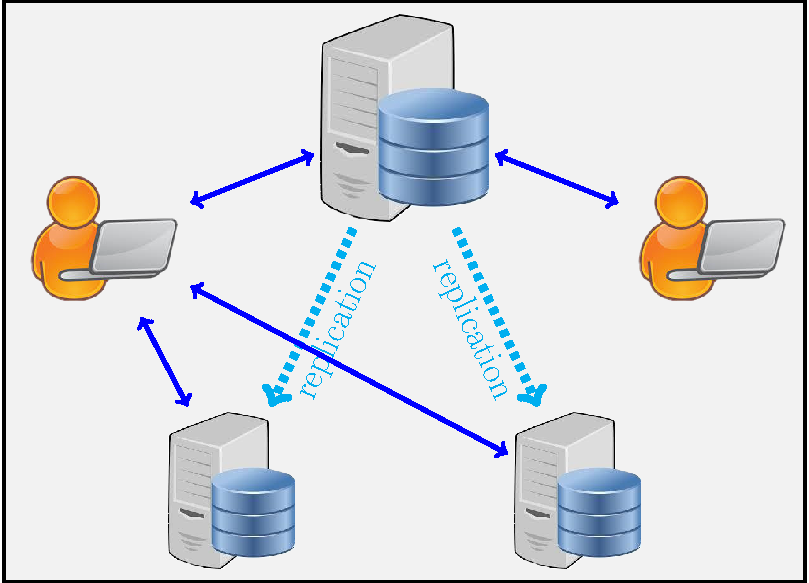
\includegraphics[scale = 0.30]{figs/master-slave.pdf}}; 
  \node (master-slave-right) [] at (5, 3) {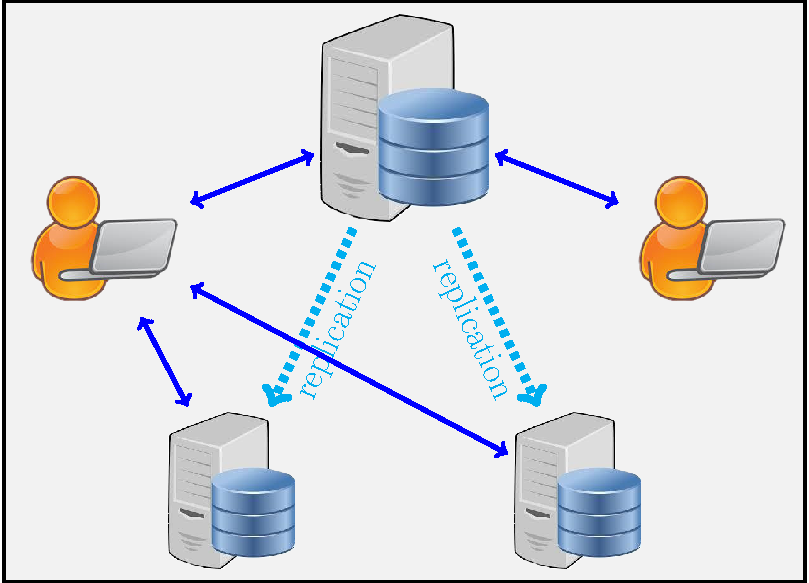
\includegraphics[scale = 0.30]{figs/master-slave.pdf}}; 
  \node (master-slave-below) [] at (2, -3) {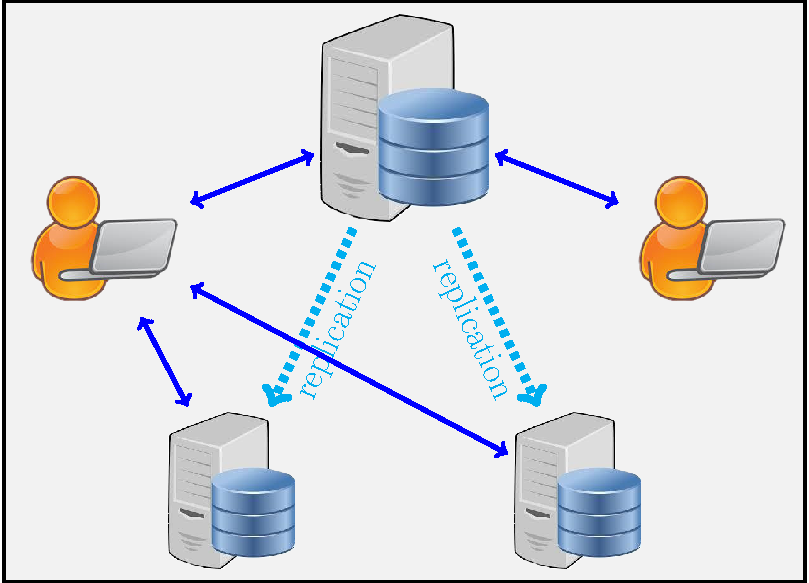
\includegraphics[scale = 0.30]{figs/master-slave.pdf}}; 

  % connection
  \draw [connection] (master-slave-left) to (master-slave-right);
  \draw [connection] (master-slave-right) to (master-slave-below);
  \draw [connection] (master-slave-left) to (master-slave-below);

  % magnified master-slave
  \node (master-slave) [] at (-7, -6) {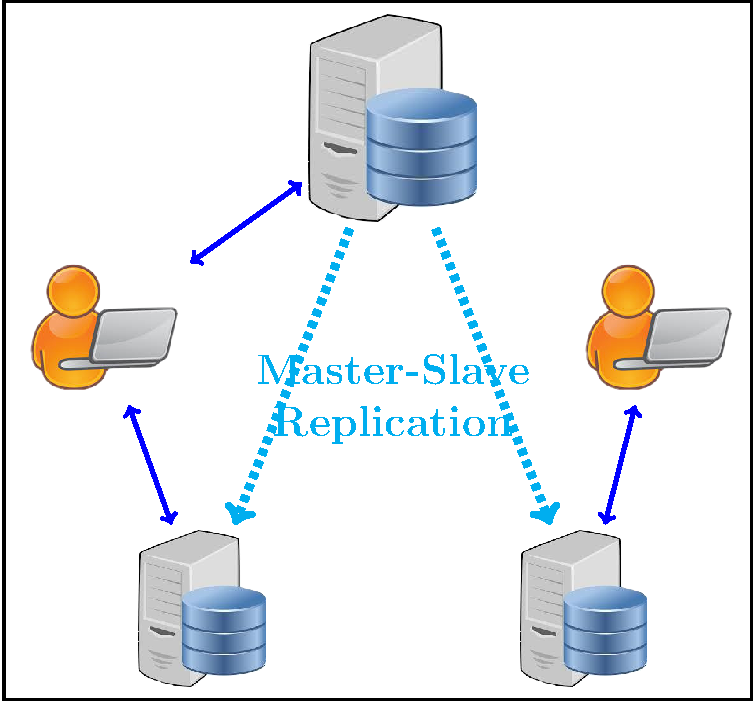
\includegraphics[scale = 0.60]{master-slave.pdf}}; 
  % magnification
  \draw [magnify] (master-slave-left) to (master-slave.north west);
  \draw [magnify] (master-slave-left.south east) to (master-slave.north east);
\end{tikzpicture}
\end{document}
